
	\section{Foreword}
		
	This thesis touches on the subjects of category theory and \emph{non-classical} mathematical logic.
 	It aims to study the \emph{Topoi} semantics of a particular \emph{non classical} logic named Gödel-Dummett Logic. \newline
	To introduce what Gödel-Dummett Logic is we first give an account (guided by \cite{goldblatt} \& \cite{awodey}) of what \emph{Intuitionistic Propositional Logic} and more broadly \emph{Intuitionism} is. 
	\newline
	\newline
%	CHECK
	(An introduction to the basic notions of category theory and mathematical logic is not given in this work.
	For this we refer to \cite{awodey},\cite{maclane},\cite{goldblatt} among others)
	

	\newpage
	
	\section{A Non-Classical World}
	
	\emph{Intuitionistic} or \emph{constructive} logic is commonly described as \emph{classical} logic without Aristotle's \emph{law of excluded middle}, a.k.a. \emph{tertium non datur}:
	\begin{definition}
		(LEM) : $A \lor \neg A$.
	\end{definition} 
	Or equivalently without the law of double negation elimination \footnote{used for \emph{reductio ad absurdum} proofs.}:
	\begin{definition}
		(DNE) : $\neg \neg A \Rightarrow A$.
	\end{definition}
	L.E.J. Brouwer in the first half of the twentieth century observed that (LEM) was abstracted from finite to infinite situations without much justification.\newline Take the following statement about the existence of infinitely many twin primes a.k.a. the \emph{twin prime conjecture} $\mathcal{P}$ in number theory:
	\begin{gather*}
		\forall x \in \mathbb{N} \; (A(x) \lor \neg A(x)) \\
		A(x) := \exists y \in \mathbb{N} ( (y > x) \land (prime(y) \land prime(y+2)) )
	\end{gather*}
	The problem with this assertion is that the \emph{twin prime conjecture} $\mathcal{P}$ like many other unsolved problems in Mathematics has not yet been proven or dis-proven so there is no proof either of $\mathcal{P}$ or $\neg \mathcal{P}$ and hence at this present \emph{state of knowledge} there can be no \emph{constructive} or \emph{effective} proof of $\mathcal{P} \lor \neg\mathcal{P}$. \newline For Brouwer and constructivists alike the claim of $\mathcal{P} \lor \neg\mathcal{P}$ is simply not acceptable. The crucial difference with the classical case is that formulae are only considered \emph{true} when we have proof or direct \emph{evidence of truth}. \newline
	This \emph{reductive} notion of truth has not been without controversy. Doing away with (LEM) or (DNE) is problematic as they are so commonly used in mathematical practice. \newline
	 For example consider a \emph{non-constructive} proof of the statement: "there exist irrational numbers $a,b$ such that $a^b$ is rational".
	 \begin{prop}
	 	$\exists\; a,b \in \mathbb{R} \setminus \mathbb{Q} : a^b \in \mathbb{Q}$.
	 \end{prop}
 \begin{proof}
 	$\sqrt{2}^{\sqrt{2}}$ is either rational or irrational. \newline
 	 In the first case we take $a = b = \sqrt{2}$. \newline
 	In the second case we take $a = \sqrt{2}^{\sqrt{2}}, b= \sqrt{2}$ and we are done.
 \end{proof}
 What's wrong? \newline
	Note that in the above proof the status of $\sqrt{2}^{\sqrt{2}}$ is \emph{undefined} and hence no \emph{constructive} proof is given for its rationality or lack thereof. \newline
	Definitive evidence of the irrationality of $\sqrt{2}^{\sqrt{2}}$ has been given by the Gelfond-Schneider Theorem which establishes \emph{constructively} that for any complex algebraic numbers $a,b \neq 1$ with $b$ irrational, $a^b$ is in fact a transcendental and hence irrational number. So the original statement has a \emph{constructive} proof.\newline 

	The \emph{BHK-interpretation} named after Brouwer,Heyting and Kolmogorov provides a framework for \emph{intuitionistic logic}.\newline In classical logic the meaning of statements is given by stating for example the following \emph{truth conditions}: 
	\begin{itemize}
		\item $\phi \land \chi$ is true iff $\phi$ is true and $\chi$ is true.
		\item $\phi \lor \chi$ is true iff $\phi$ is true or $\chi$ is true.
		\item $\neg \phi$ is true iff $\phi$ is not true.
	\end{itemize}
	In the BHK-interpretation the notion of \emph{proof}\footnote{not to be construed as syntactic or formal proof but as intuitive/informal proof or convincing mathematical argument.} replaces that of classical \emph{truth}.
	The usual logical formulae are now interpreted as:
	\begin{itemize}
		\item No proof of \emph{false} $\bot$ exists. 
		\item a proof of $\phi \;\land\; \chi$ consists of a pair of proofs, i.e., \newline   "$< \text{proof of } \phi$ ; $\text{proof of } \chi >$".
		\item a proof of $\phi \lor \chi$ is either a proof of one or the other, i.e., \newline  "proof of $\phi$ $|$ a proof of $ \chi $".
		\item a proof of $\phi \Rightarrow \chi $ consists of a \emph{method of converting} a proof of $\phi$ into a proof of $\chi$
		\item a proof of $\neg \phi$ consists of a \emph{method of converting} a proof of $\phi$ into a proof of \emph{false} (in other words "$\phi$ has no proof").
	\end{itemize}
	Moving on to first order logic and quantifiers if we assume the variables to range over a domain \emph{D}:
	\begin{itemize}
		\item a proof of $\forall x A(x)$ is a \emph{construction} that transforms any $d \in D$ into a proof of $A(d)$.
		\item a proof of $\exists x A(x)$ is a pair $<d$ ; $\text{proof of } A(d) >$.
	\end{itemize}
	
	
	How do we now formalize Intuitionistic Logic starting from the propositional layer?

	\newpage

	\section{From \textbf{IPL} to \textbf{CPL}}
	
	We begin with a presentation of the basic \emph{syntax} of \emph{Intuitionistic Propositional Logic} or \textbf{IPL}. \newline
	We do this by specifying a \emph{Formal Language} presented as an \emph{alphabet} composed of a denumerable set of propositional variables $\textbf{Prop}:=\{..,p,q,r,..\}$ and the connectives symbols $\neg, \land, \lor, \Rightarrow$. \footnote{we could also add symbols for brackets (, ) } 
	\newline
	We define \emph{inductively} Formulae $\mathbf{Form} = \{\alpha,\beta,..\phi,\chi,\psi,..\}$ in the following way:
	\begin{definition}[propositional formula]
		$\mathbf{Form}$ := $p$ $|$ $\bot$ $|$ $ F \land F $ $|$ $ F \lor F $ $|$ $ F \Rightarrow F $.
		\begin{enumerate}[label=\roman*]
			\item $\bot \in \mathbf{Form}$.
			\item  If $p\in \mathbf{Prop}$ then $p \in \mathbf{Form}$.
			\item  If $\alpha, \beta \in \mathbf{Form}$ then $(\alpha \land \beta) \in \mathbf{Form}$.
			\item  If $\alpha, \beta \in \mathbf{Form}$ then $(\alpha \lor \beta) \in \mathbf{Form}$.
			\item  If $\alpha, \beta \in \mathbf{Form}$ then $(\alpha \Rightarrow \beta) \in \mathbf{Form}$.
		\end{enumerate}
	\end{definition} 
	The constant $\bot$ represents falsity, $\land$ conjunction, $\lor$ disjunction and $\Rightarrow$ implication.
	We also define the following operators for truth, negation and double implication respectively:
	\begin{definition}
		$\top$ := $\bot \Rightarrow \bot  \;\;$,	$\; \neg \alpha$ := $\alpha \Rightarrow \bot \;\;$,	$\; \alpha \Leftrightarrow \beta$ := $(\alpha \Rightarrow \beta) \land (\beta \Rightarrow \alpha)$.
	\end{definition}

	We characterize \emph{\textbf{IPL}} by its axioms. \newline
	 The axioms for \textbf{IPL} are instances of the following schemata: \newline (Here \{\ A,B,C,..\} are meta-variables/placeholders for any propositional formula).
	
		\begin{enumerate}
			\item $ A \Rightarrow (A \land A) $.
			\item $ (A \land B) \Rightarrow (B \land A) $.
			\item $ (A \Rightarrow B) \Rightarrow ((A \land C) \Rightarrow (B \land C)) $.
			\item $ ((A \Rightarrow B) \land (B \Rightarrow C)) \Rightarrow (A \Rightarrow C) $.
			\item $ B \Rightarrow (A \Rightarrow B) $.
			\item $ (A \land (A \Rightarrow B)) \Rightarrow B $.
			\item $ A \Rightarrow (A \lor B) $.
			\item $ (A \lor B) \Rightarrow (B \lor A) $.
			\item $ ((A \Rightarrow C) \land (B \Rightarrow C)) \Rightarrow ((A \lor B) \Rightarrow C) $.
			\item $ \neg A \Rightarrow (A \Rightarrow B) $.
			\item $ ((A \Rightarrow B) \land (A \Rightarrow \neg B)) \Rightarrow \neg A $.
		\end{enumerate}
				
	Having specified the axioms, now we introduce a \emph{Propositional Calculus}\footnote{due to \emph{A. Heyting}.} for \textbf{IPL}. 
	We do this by defining a relation of \emph{entailment} or  \emph{(syntactic) derivation} between formulae
	 $\vdash$ .  \newline
	All we need to specify this \emph{derivation} is a single rule of inference that is \emph{the rule of detachment} a.k.a. \emph{Modus Ponens} [MP] .
	
	\begin{definition}[MP] For every $\alpha,\beta \in \mathbf{Form}$: \newline
		If $\vdash \alpha$ and $\vdash (\alpha \Rightarrow \beta)$, then $\vdash \beta$.
		 \newline
		which means: 
		\emph{"From $\alpha$ and $\alpha \Rightarrow \beta$ one can derive $\beta$".}
	\end{definition}
	
	$\textbf{TH}_{\textbf{IPL}}$, i.e., the \emph{Theorems} for \textbf{IPL} or \emph{provable} formulae in \textbf{IPL} denoted simply by $\vdash \phi$ \footnote{one could also use the notation $\vdash_{\textbf{IPL}}$. However we will refrain from doing so if the context is unambiguous.} are defined as all the formulae that one can derive or \emph{deduce} from $\top$ "truth" or from any instance of the axiom schemata of \textbf{IPL} in a \emph{finite} number of steps using [MP].
	\newline The relation $\alpha \vdash \beta$ in this context is characterized as $\vdash (\alpha \Rightarrow \beta)$.
	\newline
		
		
		The \emph{algebraic Semantics} for \textbf{IPL} can be obtained through the construction of a \emph{Lindenbaum-Tarski algebra} $\mathcal{A}$. \newline
		$\mathcal{A}$ is formed by taking the equivalence classes of formulae $\phi$ by the \emph{double-entailment} relation ($\phi \dashv\vdash \chi$ means "$\phi\vdash\chi$ and $\chi\vdash\phi$"):

\[ \phi \equiv \chi \text{ iff } \phi \dashv\vdash \chi\] 


		Furthermore $\mathcal{A}$ admits a well defined ordering given by entailment:
		\begin{definition}
			$[\phi] \leq [\chi] \;$	iff		$\; \phi \vdash \chi $.
		\end{definition}
		We then define the following operations in $\mathcal{A}$ induced by the logical connectives:
		\begin{itemize}
			\item $1 := [\top]$.
			\item $0 := [\bot]$.
			\item $[\phi] \land [\chi] := [\phi \land \chi]$.
			\item $[\phi] \lor [\chi] := [\phi \lor \chi]$.
			\item $[\phi] \Rightarrow [\chi] := [\phi \Rightarrow \chi]$.
	\end{itemize}

	\begin{definition}
		$\mathcal{A}$ := $(\textbf{Form}/\equiv\;, \leq)$.
	\end{definition}
	Since for every $\phi \in \textbf{Form}$ $(\bot \vdash \phi)$ and $(\phi \vdash \top)$ it follows that
	$\mathcal{A}$ is a bounded \emph{lattice} with minimum  $0 = [\bot]$ and maximum $1 = [\top]$.

\begin{prop}
	A formula $\phi$ is \emph{provable} $\top \vdash \phi$ iff $[\phi] = 1$.
\end{prop}
 		$\mathcal{A}$ with these operations is a \emph{Heyting algebra}. \newline
 		The class of Heyting algebras will be denoted by $\mathbf{HA}$. \newline
 		 What exactly is a \emph{Heyting algebra}?
 	\newline
 		A \emph{Heyting algebra} $\mathcal{H}$ is first of all a \emph{partially ordered set}, a.k.a. \emph{poset} \footnote{recall that this means that the ordering is \emph{reflexive,antisymmetric and transitive}.. not necessarily \emph{total}..}
 		$(\mathcal{H}, \leq)$ endowed with constants 0,1, binary operations \emph{join} $\lor$ and \emph{meet} $\land$
 		that form a \emph{bounded lattice}. For this the following must hold for all $a,b,c \in \mathcal{H}$:
 		 		\begin{enumerate}
 			 			\item $0 \leq a$.
 			 			\item $a \leq 1$.
 			  			\item $a \lor b \leq c \;$ iff $\;a \leq c$ and $b \leq c$.
 						\item $c \leq a \land b \;$ iff $\;c \leq a$ and $c \leq b$.
 				\end{enumerate} 
 	
 		\begin{definition}[Heyting algebra]\label{heytingalg}
 		The bounded lattice $(\mathcal{H}, \lor, \land, 0, 1)$ is said to be a \emph{Heyting algebra} if it admits a binary operator $\Rightarrow$ for which $(a \Rightarrow b) \in \mathcal{H}$, a.k.a. an \emph{exponential element}\footnote{or \emph{pseudo-complement of a with respect to b}.} such that:\newline
 			For every $a,b,c \in \mathcal{H}$ \newline there exists $(a \Rightarrow b) \in \mathcal{H}$  such that: 
 			\begin{equation*}
 				c \leq (a \Rightarrow b) \;\text{ iff }\; (c \land a) \leq b.
 			\end{equation*}
 		\end{definition}
 %check 
 \begin{remark}
 	The previous condition on exponential elements corresponds to the categorical notion of an \emph{adjoint pair} between the functors $(- \land a)$ and $(a \Rightarrow -)$ which gives rise to \emph{cartesian closed categories}.\footnote{see \cite{awodey} or \cite{maclane} for details.}
 \end{remark}
 		
 			This exponential element can also be taken as the \emph{greatest} element with this property, i.e.:
 		\begin{prop}
 			$a \Rightarrow b \equiv sup\{ c \in \mathcal{H} : c \land a \leq b \}$.	
 		\end{prop}
 	

For an analogue of classical negation, 
 		we can define for every $b \in \mathcal{H}$ a \emph{pseudo-complement} of b:
 		\begin{definition}[pseudo-complement]
 			$\neg b := (b \Rightarrow 0)$.
 		\end{definition}

\begin{remark}
	An equivalent categorical definition for a Heyting algebra, given in \cite{awodey}, is that of a \emph{cartesian closed poset}. 
\end{remark}
		We now specify the environment for the algebraic semantics of \textbf{IPL}:
	
		An $\mathcal{H}$-\emph{Interpretation} $\mathcal{I}: \mathbf{Prop} \rightarrow \mathcal{H}$ of \textbf{IPL} in a Heyting algebra $\mathcal{H}$, a.k.a. $\mathcal{H}$-\emph{valuation} is an \emph{assignment} of the propositional variables $p,q,r..$ of $\mathbf{Prop}$ to elements of $\mathcal{H}$ denoted by $\llbracket p \rrbracket_{\mathcal{H}}, \llbracket q \rrbracket_{\mathcal{H}}, \llbracket r \rrbracket_{\mathcal{H}}$...\newline
		From now on, if the context is clear $\llbracket - \rrbracket_{\mathcal{H}}$ will simply be denoted by $\llbracket - \rrbracket$. \newline 
		The interpretation  $\mathcal{I}$ is extended recursively to $\mathbf{Form}$:
		\begin{definition}[H.A. interpretation]
			Given an assignment $\mathcal{I}: \mathbf{Prop} \rightarrow \mathcal{H}$ with $p \mapsto \llbracket p \rrbracket$,\newline $\mathcal{I}: \mathbf{Form} \rightarrow \mathcal{H}$ is defined as follows:
			\begin{gather*}
			\llbracket \phi \land \chi \rrbracket := \llbracket \phi \rrbracket \land \llbracket \chi \rrbracket .\\
			\llbracket \phi \lor \chi \rrbracket := \llbracket \phi \rrbracket \lor \llbracket \chi \rrbracket .
			\\
			\llbracket \phi \Rightarrow \chi \rrbracket := \llbracket \phi \rrbracket \Rightarrow \llbracket \chi \rrbracket .\\
			\llbracket \neg \phi \rrbracket := \neg\llbracket\phi\rrbracket. \\
			 \llbracket \bot \rrbracket := 0. 
			 \\ \llbracket \top \rrbracket := 1.
			\end{gather*}
		\end{definition}

		We can talk about what it means for a formula $\phi$ to be \emph{valid} in $ \mathcal{H} $:
		
		\begin{definition}[validity in HA]
		$\phi$ is valid in $\mathcal{H}$ denoted by $\mathcal{H} \models \phi$ when $\llbracket \phi \rrbracket = 1$ for any chosen assignment for the $\mathcal{H}$-interpretation $\mathcal{I}$.
		\end{definition}
	
				There is a \emph{canonical} interpretation of \textbf{IPL} in $\mathcal{A}$ given simply by $\llbracket p \rrbracket := [p]$ and inductively by $\llbracket \phi \rrbracket := [\phi]$ that \emph{validates} only the provable formulae.
	
			If a formula $\phi$ is \emph{always true} it is called a \emph{tautology}:
		
		\begin{definition}[tautology in \textbf{IPL}]
			A formula $\phi$ is a \emph{tautology}\footnote{tautology in \textbf{IPL}.} or \emph{Intuitionistically valid} denoted by $\vDash \phi$ if it is valid in every Heyting algebra $\mathcal{H}$.
		\end{definition}	
		
		\begin{remark}
			If a formula $\phi$ is a \emph{tautology}, one has in particular in $\mathcal{A}$ that $1 = \llbracket \phi \rrbracket = [\phi]$ and so $\vdash \phi$. 
		\end{remark}	
		
		We can show that all axioms are tautologies and that the inference rule (MP) \emph{preserves validity}, i.e., "if $\vDash \phi$ and $\vDash (\phi \Rightarrow \psi)$ then $\vDash \psi$". \newline
		This gives us the following result:
		
		\begin{prop}
			$\vdash \phi$ iff  $\vDash \phi$, i.e., "$\phi$ is provable\footnote{in \textbf{IPL}.} iff $\phi$ is \emph{intuitionistically} valid".
		\end{prop}
		
		which means that:
		
		\begin{prop}
			\begin{equation*}
				\vdash_{IPL} \alpha \text{ iff } H \vDash \alpha \text{ for all } H \in \mathbf{HA}.
			\end{equation*}
			,i.e. , \emph{Heyting algebras} provide \emph{sound} and \emph{complete} semantics for \textbf{IPL}
		\end{prop}

		What about \emph{Classical Propositional Logic} or \textbf{CPL}? 
	\newline
	We keep the same syntax and calculus used in the intuitionistic case but add an axiom "$12. \; (A \lor \neg A)$" which corresponds to the Law of Excluded Middle (LEM).\newline
	We use the following notation to show this fact:
	
		\[ \textbf{CPL} = \textbf{IPL} + (A \lor \neg A) \]
 
	This time a provable formulae in \textbf{CPL}, i.e., $\vdash_{CPL} \phi$ \footnote{again, from now on we omit to specify $\vdash_{\textbf{CPL}}$.} can also be derived from any instance of (LEM) and thus:
	\begin{prop}
		$\textbf{TH}_\textbf{IPL} \subset \textbf{TH}_\textbf{CPL}$.
	\end{prop}
	We will see that this inclusion is strict. \newline
	
		Now, we can construct the Lindenbaum-Tarski algebra $\mathcal{A'}$ as before by taking the equivalence classes of formulae by double entailment and repeating the same definitions for its ordering and operations. 
		The following still holds:
		\begin{prop}
			A formula $\phi$ is \emph{provable} $\vdash \phi$ iff $[\phi] = 1$.
		\end{prop}
		$\mathcal{A'}$ is a special case of a \emph{Heyting algebra} called a \emph{Boolean algebra}. \newline
		What is a Boolean algebra? 
		\begin{definition}
			A Boolean algebra $(\mathcal{B}, \lor, \land, \Rightarrow, 0, 1)$ is a Heyting algebra where for every $a \in \mathcal{B}$ the pseudo-complement of $a$, i.e., $\neg a$ is a \emph{complement} of $a$ which means:
			\begin{enumerate}
				\item $a \land (\neg a) = 0$.
				\item $a \lor (\neg a) = 1$. 
			\end{enumerate}
		\end{definition}
				
		We denote the class of Boolean algebras by $\mathbf{BA}$. \newline
	\newline
		 			Note that with these definitions
		 					every Boolean algebra is a Heyting algebra though in general a Heyting algebra need not be Boolean. In fact we will see examples in which this is the case.
		 			
		The algebraic semantics for \textbf{CPL} are given in a very similar way to the classical case.
		An \emph{Interpretation}  or $\mathcal{B}$-valuation $\mathcal{V}$ of \textbf{CPL} in a Boolean algebra $\mathcal{B}$ is again an assignment of propositional variables to elements of $\mathcal{B}$ denoted by $\llbracket p \rrbracket, \llbracket q \rrbracket, \llbracket r \rrbracket$.. The interpretation extends recursively to all formulae as before with the addendum $\llbracket \neg \phi \rrbracket = \neg \circ \llbracket \phi \rrbracket$.
		
		More commonly, we deal with a \emph{valuation} $\mathcal{V}$ in the two-element Boolean algebra of \emph{truth values} $\mathbb{2}=\{0 < 1\}$ which specifies a \emph{value assignment}, i.e., any function $V : \textbf{Prop} \rightarrow \mathbb{2}$. Also by our recursive definition of $\mathcal{V}$:
		
		\begin{remark}
			$V : \textbf{Prop} \rightarrow \mathbb{2}$ is \emph{lifted} in a unique way to $V : \textbf{Form} \rightarrow \mathbb{2}$ a so-called \emph{truth}-function on any formula.
		\end{remark}

		We can talk about what it means for a formula $\phi$ to be \emph{valid} in $ \mathcal{B} $:
		
		\begin{definition}[validity in BA]
			$\phi$ is valid in $\mathcal{B}$ denoted by $\mathcal{B} \models \phi$ when $\llbracket \phi \rrbracket = 1$ for any chosen assignment for the $\mathcal{B}$-valuation $\mathcal{V}$.
		\end{definition}
	There is a \emph{canonical} interpretation of \textbf{CPL} in $\mathcal{A}$ given simply by $\llbracket p \rrbracket := [p]$ and inductively by $\llbracket \phi \rrbracket := [\phi]$ that \emph{validates} only the provable formulae.
		
		If a formula $\phi$ is \emph{always true} it is called a \emph{tautology}:
		
		\begin{definition}[tautology in \textbf{CPL}]
			A formula $\phi$ is a \emph{tautology}\footnote{tautology in \textbf{CPL}.} or \emph{classically valid} denoted by $\vDash \phi$ if it is valid in every Boolean algebra $\mathcal{B}$.
		\end{definition}	
				
In a similar fashion as before, we conclude that:
		
		\begin{prop}
			\begin{equation*}
				\vdash_{CPL} \alpha \text{ iff } B \vDash \alpha \text{ for all } B \in \mathbf{BA}.
			\end{equation*}		,i.e. ,
			\emph{Boolean algebras} provide \emph{sound} and \emph{complete} semantics for \emph{Classical Propositional Logic}
		\end{prop}
		
		
		To sum up:
		\begin{itemize}
			\item Heyting algebras provide a (sound and complete) algebraic semantics for Intuitionistic Propositional Logic (\textbf{IPL}).
			\item 	$\textbf{CPL} = \textbf{IPL} + (A \lor \neg A)$ and 	$\textbf{TH}_\textbf{IPL} \subset \textbf{TH}_\textbf{CPL}$ . 
			\item $\mathbf{BA} \subset \mathbf{HA}$ Boolean algebras are a particular class of Heyting algebras  which provide a (sound and complete) algebraic semantics for Classical Propositional Logic (\textbf{CPL}).
		\end{itemize} 
	
	
			The canonical examples of Boolean algebras are:
			
			\begin{ex}[Power-Set]
					$( \mathcal{P}(X),  \subseteq )$, i.e., the set of sub-sets, a.k.a. \emph{Power-Set} of a set $X$ with the set-inclusion partial ordering is a \emph{Boolean algebra} with $0 := \emptyset$, $1 := X$, $\lor := \cup$, $\land := \cap$ and $\neg := (\;)^\complement $.
				\end{ex}
			
			\begin{ex}[$\mathbb{2}$]
				We encountered a special case of the \emph{power-set} Boolean algebra, which corresponds to the power-set of the singleton set $\mathcal{P}(\{*\})$, i.e., the \emph{two-element} Boolean algebra of \emph{truth-values} $\mathbb{2} := \{0 < 1\}$, where $0$ and $1$ represent $false$ and $true$ respectively. \newline
				Note that here the Law of Excluded Middle (LEM) clearly holds:\newline $\mathbb{2} \models (\alpha \lor \neg \alpha)$.
			\end{ex}
			
			\begin{ex}[$free_1(B)$]
				The Boolean algebra \emph{freely generated}\footnote{this can be seen as the Lindenbaum-Tarski algebra with just one propositional variable.} by the element $p$. 
			\end{ex}
			
			\begin{figure}[h]
				\centering
				\begin{tikzpicture}[thick,scale=0.6, every node/.style={scale=0.8}]
					\node (A) at (0,0) {0};
					\node (B) at (0,3) {1};
					\draw[line width=.01in] (A) -- (B);
				
					\node (A) at (8,0) {0};
					\node (B) at (6,2) {$p$};
					\node (C) at (10,2) {$\neg p$};
					\node (D) at (8,4) {1};
					\draw[line width=.01in] (A) -- (B);
					\draw[line width=.01in] (A) -- (C);
					\draw[line width=.01in] (C) -- (D);
					\draw[line width=.01in] (B) -- (D);
				\end{tikzpicture}
				\caption{ $\mathbb{2}$ (left) and $free_1(B)$ (right). }
			\end{figure}
			
For Heyting algebras the canonical example is:

\begin{ex}[Open Sets]
	The lattice of \emph{Open Sets} $(\mathcal{O},\subseteq)$ (ordered by inclusion) of a topological space $(X,\tau)$  is a Heyting algebra with $0 := \emptyset$, $1 := X$, $\lor := \cup$, $\land := \cap$ and: \newline $U \Rightarrow V := (U^\complement \cup V)^\circ$, i.e., the \emph{largest open sub-set} of $U^\complement \cup V$. \newline
	This means that whenever $W$ is open, $W \subseteq (U^\complement \cup V)^\circ$ iff $(U \cap W) \subseteq V$.
\end{ex}

The following example shows that not every Heyting algebra need be Boolean   $\mathbf{BA} \subsetneq \mathbf{HA}$ and that 	$\textbf{TH}_\textbf{IPL} \subsetneq \textbf{TH}_\textbf{CPL}$ :

\begin{ex}[The case of $\neg\neg a \neq a$]
	Note that in the Heyting algebra of Open Sets the \emph{pseudo-complement} of any open set corresponds to the interior of its complement, i.e., $\neg U := (U \Rightarrow \emptyset) = (U^\complement)^\circ$. \newline
	Note that in a Boolean algebra "$\neg\neg a = a$" must hold for every element. \newline
	$a \leq \neg \neg a$ holds in $(\mathcal{O},\subseteq)$ since $\neg \neg a = ((a \Rightarrow 0) \Rightarrow 0)$ and $a \land (a \Rightarrow 0) \leq 0$ by \emph{evaluation}. \newline\newline
	The converse $\neg\neg a \leq a$ however in general does not hold.\newline
	Take for example the open sets in $[0,1]$ with the induced standard topology. \newline
	By unfolding the definition of $\neg$ we obtain : $\neg\neg (0,1) = [0,1] \nsubseteq (0,1)$.\newline\newline
	Finally, if we consider (in the induced topology of $[0,1]$)  the open set $[0,1/2)$ and  $[0,1/2)^\complement = (1/2,1]$ we observe that $[0,1/2) \cup [0,1/2)^\complement \subsetneq [0,1]$, i.e., \newline LEM $A \lor \neg A$ is not \emph{intuitionistically} valid. In other words:
	\begin{equation*}
		\nvdash_{IPL} A \lor \neg A.
	\end{equation*}
	 
\end{ex}
	
\begin{ex}[$free_1(H)$]
		The Heyting algebra \emph{freely generated}\footnote{this again can be seen as the Lindenbaum-Tarski algebra with just one propositional variable.} by the element $p$. \newline
		This forms an infinite lattice called the \emph{Rieger-Nishimura ladder}. 
	\end{ex} 
	
	
	\begin{figure}[h]
		\centering
		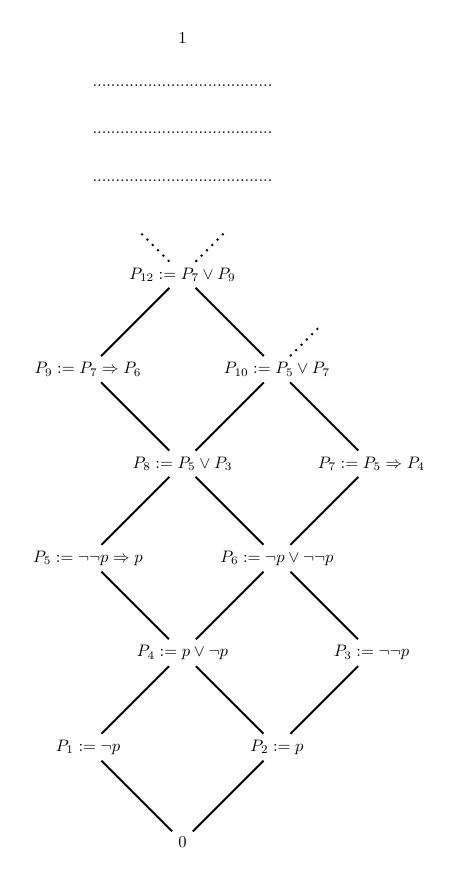
\begin{tikzpicture}[thick,scale=0.6, every node/.style={scale=0.6}]
			\node (A) at (0,0) {$0$};
			\node (B) at (-2,2) {$P_1 := \neg p$};
			\node (C) at (2,2) {$P_2 := p$};
			\node (D) at (0,4) {$P_4 := p \lor \neg p$};
			\node (E) at (4,4) {$P_3 := \neg \neg p$};
			\node (F) at (2,6) {$P_6 := \neg p \lor \neg \neg p$};
			\node (G) at (-2,6) {$P_5 := \neg \neg p \Rightarrow p$};
			\node (H) at (0,8) {$P_8 := P_5 \lor P_3$};
			\node (I) at (4,8) {$P_7 := P_5 \Rightarrow P_4$};
			\node (J) at (2,10) {$P_{10} := P_5 \lor P_7$};
			\node (J') at (3,11) {};
			\node (K) at (-2,10) {$P_{9} := P_7 \Rightarrow P_6$};
			\node (L) at (0,12) {$P_{12} := P_7 \lor P_9$};
			\node (L') at (1,13) {};
			\node (L'') at (-1,13) {};
			\node (M) at (0,14) {.......................................};
			\node (N) at (0,15) {.......................................};
			\node (0) at (0,16) {.......................................};
			\node (P) at (0,17) {$1$};
			\draw[line width=.01in] (A) -- (B);
			\draw[line width=.01in] (A) -- (C);
			\draw[line width=.01in] (B) -- (D);
			\draw[line width=.01in] (C) -- (D);
			\draw[line width=.01in] (C) -- (E);
			\draw[line width=.01in] (E) -- (F);
			\draw[line width=.01in] (D) -- (F);
			\draw[line width=.01in] (D) -- (G);
			\draw[line width=.01in] (G) -- (H);
			\draw[line width=.01in] (F) -- (H);
			\draw[line width=.01in] (F) -- (I);
			\draw[line width=.01in] (H) -- (J);
			\draw[line width=.01in] (I) -- (J);
			\draw[line width=.01in] (H) -- (K);
			\draw[line width=.01in] (K) -- (L);
			\draw[line width=.01in] (J) -- (L);
			\draw[dotted, line width=.01in] (J) -- (J');
			\draw[dotted, line width=.01in] (L) -- (L');
			\draw[dotted, line width=.01in] (L) -- (L'');
		\end{tikzpicture}
		\caption{$free_1(H)$ displayed as the \emph{Rieger-Nishimura ladder} in which we used auxiliary meta-variables $P_n$ to label the nodes. }
	\end{figure}
	
	
	
	
	
\newpage
	
	\section{States of Knowledge}
	
	We introduce, following \cite{goldblatt}, a new semantics for IPL given by \emph{S.Kripke} which will give us a better insight into our area of study. \newline
	The structure we shall be concerned with is a poset \textbf{P} called a \emph{Kripke Frame}  which represents a finite set of \emph{possible worlds}, a.k.a. \emph{states of knowledge} with a so-called \emph{temporal ordering}.\newline
	(Propositional) Formulae are now interpreted as sub-sets of this poset which represents the states at which the sentence is \emph{true} . \newline
	A formula, we shall see, is not true or false per se but rather \emph{true at a certain state of knowledge} and once true remains true in all \emph{future states}, i.e., we have \emph{the persistence of truth in time}. \newline
	This accords well with the intuitionistic point of view in which a formula is true when its truth has been \emph{constructively determined} at some state or \emph{stage} and \emph{constructive knowledge} once established lasts forever. \newline
	Note that this temporal ordering of states of knowledge need not be \emph{linear}. This embodies the idea that from the \emph{present} state, there might be more than one possible \emph{future} state. Consider for example a world in which \emph{Fermat's Last Theorem} is determined to be true and one in which it is shown to be false. 
	
	\begin{definition}[Kripke Frame]
	A Kripke Frame $\textbf{P} := (P, \sqsubseteq)$ is a finite set of \emph{possible worlds}
	ordered by a partial (so-called \emph{temporal}) ordering $\sqsubseteq$.
	\end{definition} 
	
	Having fixed a Kripke Frame,
	we introduce the notion of an \emph{hereditary} sub-set of \textbf{P}:
	
	\begin{definition}[hereditary sub-set]
		$A \subseteq P$ is \emph{hereditary} if it is \emph{upwards-closed} under $\sqsubseteq$, i.e., if $p \in A$ and $p \sqsubseteq q$ we have that $q \in A$. \newline
		The collection of all these hereditary up-sets will be denoted by $\textbf{P}^+$.
	\end{definition}  
	
	Semantics is now given by assigning to each propositional variable a hereditary sub-set by a \textbf{P}-valuation $\mathcal{V}$, i.e., a function $\mathcal{V} : \textbf{Prop} \rightarrow \textbf{P}^+$. 
	
	\begin{remark}
		$\mathcal{V}(\textbf{p})$ formalizes the idea of \emph{"the set of states at which $\textbf{p}$ is determined to be true"} and being an hereditary sub-set this means that the \emph{knowledge of this truth is persistent in time}.
	\end{remark}
	
	We define a \emph{Kripke Model} $\mathcal{M}$ and give a formal definition of what it means for a formula to be \emph{true} at a particular state:
	
	\begin{definition}[Kripke Model]
		A \emph{Kripke Model} based on \textbf{P} is $\mathcal{M} := (\textbf{P}, \mathcal{V})$ where $\mathcal{V}$ is a \textbf{P}-valuation. \newline
		We define inductively a \emph{forcing relation} $\mathcal{M} \VDashA_w \alpha$ \newline, i.e., \emph{"in $\mathcal{M}$ world $w$ forces formula $\alpha$"} or also \emph{"the formula $\alpha$ is true in $\mathcal{M}$ at  $w \in P$"}:
		\begin{enumerate}
			\item $\mathcal{M} \VDashA_w \textbf{p}$ iff $w \in \mathcal{V}(\textbf{p})$.
			\item $\mathcal{M} \VDashA_w (\alpha \land \beta)$ iff $\mathcal{M} \VDashA_w \alpha$ and $\mathcal{M} \VDashA_w \beta$.
			\item $\mathcal{M} \VDashA_w (\alpha \lor \beta)$ iff either $\mathcal{M} \VDashA_w \alpha$ or $\mathcal{M} \VDashA_w \beta$.
			\item $\mathcal{M} \VDashA_w (\neg\alpha)$ iff for all $s$ such that $w \sqsubseteq s$ it is not the case that $\mathcal{M} \vDash_s \alpha$.
			\item $\mathcal{M} \VDashA_w (\alpha \Rightarrow \beta)$ iff for all $s$ such that $w \sqsubseteq s$, if $\mathcal{M} \vDash_s \alpha$ then $\mathcal{M} \vDash_s \beta$.
		\end{enumerate}
		With the expression $\mathcal{M} \vDash \alpha$, i.e., \emph{$\alpha$ is true in $\mathcal{M}$}, we indicate that $\mathcal{M} \VDashA_w \alpha$ holds for all $w \in \textbf{P}$.
	\end{definition}
	
	\begin{remark}
		The truth of $\neg \alpha$ at state $w$ means that $\alpha$ is never verified at any later stage.
	\end{remark}
	
	The notion of \emph{validity} is readily given:
	
	\begin{definition}[Kripke Validity]
		A formula $\alpha$ is valid on the frame \textbf{P}, denoted by $\textbf{P} \VDashA \alpha$, if for every model $\mathcal{M}$ based on \textbf{P} we have $\mathcal{M} \VDashA \alpha$. 
	\end{definition}
	
	Let us now consider the hereditary set of states at which $\alpha$ is \emph{true} in $\mathcal{M}$:
	
	\begin{definition}
		$\mathcal{M}(\alpha) := \{ w : \mathcal{M} \VDashA_w \alpha\}$.
	\end{definition} 
	
	Also we introduce the following operations:  
	\begin{definition}
		For any hereditary sets $S,  T$:
	\begin{gather*}
		\neg S := \{w: \text{ for all } z, \; w \sqsubseteq z, \; z \notin S\}. \\
		S \Rightarrow T := \{ w: \text{ for all } z, \; w \sqsubseteq z, \;\text{ if } z \in S \text{ then } z \in T \}.
	\end{gather*}	
	\end{definition}
	
	
	With these definitions: 
	\begin{prop}
		For any hereditary $S,T,U$: \newline
		$ U \subseteq (S \Rightarrow T) $ iff $ (S \cap U) \subseteq T $ and
		$\neg S = S \Rightarrow \emptyset$.
	\end{prop}
	
	The definition of a Kripke Model we gave earlier can be given in an equivalent fashion by requiring that:
	
	\begin{enumerate}[label=(\roman*)]
		\item $\mathcal{M}(\textbf{p}) = \mathcal{V}(\textbf{p})$.
		\item $\mathcal{M}(\alpha \land \beta) = \mathcal{M}(\alpha) \cap \mathcal{M}(\beta)$.
		\item $\mathcal{M}(\alpha \lor \beta) = \mathcal{M}(\alpha) \cup \mathcal{M}(\beta)$.
		\item $\mathcal{M}(\neg\alpha) = \neg\mathcal{M}(\alpha)$.
		\item $\mathcal{M}(\alpha \Rightarrow \beta) = \mathcal{M}(\alpha) \Rightarrow \mathcal{M}(\beta)$.
	\end{enumerate}
	
	Note that since the intersection $\cap$ and union $\cup$ of hereditary sets is hereditary:
	
	\begin{thm}
		$(\textbf{P}^+, \subseteq )$ with the operations $\cap$,$\cup$ and $\Rightarrow$ is a Heyting algebra.
	\end{thm}
	
	Any \textbf{P}-valuation $\mathcal{V}: \textbf{Prop} \rightarrow \textbf{P}^+$ can now be seen as a $\textbf{P}^+$-valuation for the Heyting algebra  $\textbf{P}^+$. \newline
	We have $\mathcal{V}(\textbf{p}) = \mathcal{M}(\textbf{p})$ and by extending  $\mathcal{V}$ inductively to arbitrary formulae\footnote{$\mathcal{V}(\alpha \land \beta) := \mathcal{V}(\alpha) \cap \mathcal{V}(\beta)$, $\mathcal{V}(\alpha \lor \beta) := \mathcal{V}(\alpha) \cup \mathcal{V}(\beta)$, $\mathcal{V}(\alpha \Rightarrow \beta) := \mathcal{V}(\alpha) \Rightarrow \mathcal{V}(\beta)$ etc..}:
	\begin{lem}
		$\mathcal{M}(\alpha) = \mathcal{V}(\alpha)$ for any formula $\alpha$.
	\end{lem}
	Putting all this together:
	
	\begin{prop}
		$\mathcal{M} \VDashA \alpha$ iff $\mathcal{M}(\alpha)=P$ iff $\mathcal{V}(\alpha)=P$.
	\end{prop}
	
	Also, since $P$ is the top element of the lattice $\textbf{P}^+$, we obtain a link between \emph{Kripke validity} on the frame \textbf{P} and \emph{Heyting algebra validity} on $\textbf{P}^+$:
	
	\begin{thm}
		$\textbf{P} \VDashA \alpha$ iff $\textbf{P}^+ \models \alpha$.
	\end{thm}
	
Returning to the Semantics of IPL, we have the following result:
	
	\begin{thm}
		 \begin{equation*}
			\vdash_{IPL} \alpha\text{ iff }\textbf{P} \VDashA \alpha \text{ for any frame }\textbf{P}.
		\end{equation*} i.e.,
		Kripke Semantics is sound and complete for IPL.
\end{thm}

	Soundness comes from the fact that if $\vdash_{IPL} \alpha$ then for any Heyting algebra $H$ we have $H \models \alpha$. 
	For any frame \textbf{P} we thus have $\textbf{P}^+ \models \alpha$ and so $\textbf{P} \VDashA \alpha$. \newline
	For Completeness, for $p\in \textbf{P}$ we introduce the set of sentences \emph{known to be true at p}, a.k.a. the \emph{extension} of $p$ :
	
	\begin{definition}[extension of $p$]
		 $\Gamma_p := \{ \alpha : \mathcal{M} \VDashA_p \alpha \}$ denotes the \emph{extension} of $p$.
		This set of sentences satisfies the following properties:
		\begin{enumerate}
			\item (soundness) If $\vdash_{IPL} \alpha$ then $\alpha \in \Gamma_p$.
			\item (closure under MP) If $\vdash_{IPL} \alpha \Rightarrow \beta$ and $\alpha \in \Gamma_p$ then $\beta \in \Gamma_p$.
			\item (consistency) There exists an $\alpha$ such that $\alpha \notin \Gamma_p$.
			\item (primality) If $\alpha \lor \beta \in \Gamma_p$ then $\alpha \in \Gamma_p$ or $\beta \in \Gamma_p$.
		\end{enumerate}
	\end{definition}
	
		$\Gamma_p$ is also called a \emph{state-description} of the state $p\in \textbf{P}$ by discerning the sentences known to be true at $p$.
	
	\begin{definition}[full set]
		A set $\Gamma \subseteq \textbf{Form}$ that satisfies the previous conditions 1.-4. is called \emph{full}.
	\end{definition}
	
	We can now introduce the so-called \emph{canonical model} for IPL:
	
	\begin{definition}[canonical frame]
		The canonical frame for IPL is the collection of \emph{all} full sets ordered by inclusion $\textbf{P}_{IPL} := (P_{IPL}, \subseteq)$.
	\end{definition}
	
	\begin{definition}[canonical model]
		The canonical model for IPL is given by $\mathcal{M}_{IPL}:=(\textbf{P}_{IPL}, V_{IPL})$ where:
		\begin{equation*}
			V_{IPL} : \textbf{p}_i \mapsto \{\Gamma: \textbf{p}_i \in \Gamma\}
		\end{equation*}
		i.e., the canonical valuation assigns to every proposition the set of full sets that contain it.
	\end{definition}
	
	If we add the following results:
	
	\begin{lem}
		$\mathcal{M} \VDashA_\Gamma \alpha$ iff $\alpha \in \Gamma$.
	\end{lem}
	
	\begin{lem}[Lindenbaum]
		$\vdash_{IPL} \alpha$ iff $\alpha$ is a member of every full set.
	\end{lem}
	
	We obtain the desired completeness result:
	
	\begin{thm}
		$\vdash_{IPL} \alpha$ iff $\mathcal{M}_{IPL} \VDashA \alpha$ iff $\textbf{P}_{IPL} \VDashA \alpha$.
	\end{thm}
	
	Kripke Semantics can also provide a \emph{topological} interpretation of \emph{intuitionism} as for any frame \textbf{P} the hereditary sets $\textbf{P}^+$ form a \emph{topology}:
	
	\begin{prop}
		$\textbf{P}^+$ is the Heyting algebra of Open Sets for the topology just described.\newline
		In particular one has $\neg S = (S^\complement)^\circ$ the largest hereditary subset of $S^\complement$ and 
	\end{prop}
	

	Another nice feature of Kripke semantics is that one can determine the validity (or lack thereof) of formulae by looking at the \emph{structure} of the frames. \newline 
	
To illustrate this point,
	a few simple examples of  Kripke Models are illustrated:
		
	\begin{ex}
		$\mathcal{T} := \{ \textbf{2}, \mathcal{V} \}$. \newline
		Where $\textbf{2} :=\{ 0 < 1 \}$ and  $\mathcal{V}: \textbf{p} \mapsto {1}$.\newline
		We can ask ourselves if the instance of LEM "$\textbf{p} \lor \neg \textbf{p}$" is valid on this frame.\newline
		The answer is \emph{no}. To see this:\newline
		Note that $\mathcal{T} \nVDash_0 \textbf{p} $ but $\mathcal{T} \VDashA_1 \textbf{p} $ with $0\leq 1$.\newline
		So, by definition we also have  $\mathcal{T} \nVDash_0 \neg\textbf{p} $ and so  $\mathcal{T} \nVDash_0 (\textbf{p} \lor \neg \textbf{p}) $ i.e., LEM is not valid on this frame.
	\end{ex}
	
	
	\begin{figure}[h]
		\centering
		\begin{tikzpicture}[thick,scale=0.6, every node/.style={scale=0.8}]
			\node (A) at (0,0) {$\bigcdot_0$};
			\node (B) at (0,3) {$\bigcdot_1$};
			\node (b) at (-1,3) {\textbf{p}};
			\draw[line width=.01in] (A) -- (B);
			\end{tikzpicture}
		\caption{ Kripke Model $\mathcal{T}$. The propositions \emph{true} at $0,1$ are listed beside the node labeled by the state $0,1$.}
	\end{figure}
	
	
	
	\begin{ex}
		$\mathcal{K} := \{ \textbf{W}, \mathcal{V} \}$. \newline
		Where $\textbf{W} :=\{r < w_1 < w_3, r < w_2 < w_3\}$ and  $\mathcal{V}: \textbf{p} \mapsto {w_1,w_3}, \textbf{q} \mapsto {w_2,w_3 }$. \newline
		Similarly as before the LEM is not valid on this frame though its weaker version\footnote{wLEM := $(\neg \alpha \lor \neg \neg \alpha)$.} $ \neg\textbf{p} \lor \neg\neg \textbf{p} $ holds. \newline
		
		What can we say of the classically valid \emph{pre-linearity axiom}, i.e., \newline  "$(\alpha \Rightarrow \beta) \lor (\beta \Rightarrow \alpha)$"? \newline
		Since $\mathcal{T} \VDashA_{w_1} \textbf{p} $, $\mathcal{T} \nVDash_{w_1} \textbf{q} $ and $\mathcal{T} \VDashA_{w_1} \textbf{q} $, $\mathcal{T} \nVDash_{w_1} \textbf{p} $ we have that: \newline$\nvDash_r (\textbf{p} \Rightarrow \textbf{q}) \lor (\textbf{q} \Rightarrow \textbf{p})$.\newline
		This tells us that the pre-linearity axiom is not valid on this frame and thus is not intuitionistically valid, i.e., 
		\begin{equation*}
			\nvdash_{IPL} (\alpha \Rightarrow \beta) \lor (\beta \Rightarrow \alpha).
		\end{equation*}
		However this formula is valid for example on the previous frame $\mathcal{T}$.   
	\end{ex}
	
	
	\begin{figure}[h]
		\centering
		\begin{tikzpicture}[thick,scale=0.6, every node/.style={scale=0.8}]
			\node (A) at (0,0) {$\bigcdot_r$};
			\node (B) at (-3,3) {$\bigcdot_{w_1}$};
			\node (b) at (-4,3) {\textbf{p}};
			\node (C) at (3,3) {$\bigcdot_{w_2}$};
			\node (c) at (4,3) {\textbf{q}};
			\node (D) at (0,6) {$\bigcdot_{w_3}$};
			\node (d) at (-1.5,6) {\textbf{p},\textbf{q}};
			\draw[line width=.01in] (A) -- (B);
			\draw[line width=.01in] (A) -- (C);
			\draw[line width=.01in] (B) -- (D);
			\draw[line width=.01in] (C) -- (D);
		\end{tikzpicture}
		\caption{ Kripke Model $\mathcal{K}$. The propositions \emph{true} at $w_i$ are listed beside the node labeled by the state $w_i$.}
	\end{figure}
	
	
We can also recover \emph{classical} validity: 
	
	\begin{ex}
		Recall the classical validity of the form $\mathbb{2} \models \alpha$, i.e., validity on the two-element Boolean algebra $\mathbb{2}=\{0<1\}$, means that $\llbracket \alpha \rrbracket = 1$ for any truth assignment of the propositional variables $V: \textbf{Prop} \rightarrow \mathbb{2}$. If we now specify: \newline  
		
		$\mathcal{C} := \{ \{ w \}, \tilde{V} \}$. \newline
		Where $\mathcal{V}: \textbf{p} \mapsto {w}$ iff $V: \textbf{p} \mapsto 1$.\newline
		So classical validity is the same as Kripke-validity on this discrete frame, i.e.,
		$\{ w \} \VDashA \alpha$ iff $\mathbb{2} \models \alpha$.
	\end{ex}
	
	
	\begin{figure}[h]
		\centering
		\begin{tikzpicture}[thick,scale=0.6, every node/.style={scale=0.8}]
			\node (A) at (0,0) {$\bigcdot_w$};
			\node (a) at (-1,0) {$\textbf{p}_i$};
		\end{tikzpicture}
		\caption{ Kripke Model $\mathcal{C}$ in which $\textbf{p}_i$ stands for all the propositions valued at 1.}
	\end{figure}
	
	
	These examples suggest the following definitions:
	
	\begin{definition}[discrete]
		The frame \textbf{P} is \emph{discrete}, i.e., has $z \sqsubseteq w$ iff $z=w$,  iff  \newline $\textbf{P} \VDashA (\alpha \lor \neg \alpha)$.
	\end{definition}
	
	
	\begin{definition}[directed]
		The frame \textbf{P} is \emph{directed}, i.e., if $z \sqsubseteq w$ and $z \sqsubseteq v$ then there exists an $s$ with $w \sqsubseteq s$ and $v \sqsubseteq s$, iff  \newline $\textbf{P} \VDashA (\neg \alpha \lor \neg \neg \alpha)$.
	\end{definition}
	
	
	\begin{definition}[weakly linear]
		The frame \textbf{P} is \emph{weakly linear}, i.e., if $z \sqsubseteq w$ and $z \sqsubseteq v$ then either $w \sqsubseteq v$ or $v \sqsubseteq w$, iff  \newline $\textbf{P} \VDashA (\alpha \Rightarrow \beta) \lor (\beta \Rightarrow \alpha)$.
	\end{definition}
	
	
	\newpage
	
		\section{An Intermediate and Fuzzy Logic}
		\label{intermediate}
The following introduction, which draws heavily from \cite{fuzzy} \& \cite{firstorder} among others, is a recollection of known results.
		As the name suggests:
		
		\begin{definition}[intermediate propositional logic]
			 An \emph{intermediate}, a.k.a. \emph{super-intuitionistic} propositional logic $\mathcal{L}$ is such that: $\textbf{Th}_{\textbf{IPL}} \subset \textbf{Th}_\mathcal{L} \subset \textbf{Th}_{\textbf{CPL}}$, i.e., its theorems include all the \textbf{IPL}-theorems and are included in the \textbf{CPL}-theorems.
			 
		\end{definition}
		
		An Intermediate Propositional Logic is Gödel-Dummett Propositional Logic $\mathcal{G}$, obtained by extending the standard \textbf{IPL} with the \emph{pre-linearity} axiom we encountered earlier:
		
		\begin{definition}
			 $\mathcal{G} := \textbf{IPL} \; + \; ((A \Rightarrow B) \lor (B \Rightarrow A))$.
		\end{definition}
	
	We will also use the following notation to express this fact:
	\begin{equation*}
		{\textbf{IPL}} \subset \mathcal{G} \subset {\textbf{CPL}}
	\end{equation*}
	
		The algebraic semantics of $\mathcal{G}$ is given by the variety, i.e., an equationally definable class, $\mathbb{G}$ of \emph{Gödel algebras}:
		
		\begin{remark} For every formula $\alpha$ one has : 
			$\vdash_{\mathcal{G}} \alpha$ iff $G \vDash \alpha$ for all $G \in \mathbb{G}$. 
		\end{remark}
		
		A Gödel algebra \emph{G} is a Heyting algebra that satisfies \emph{pre-linearity}:
	
		\begin{definition}
			 $\emph{G} := (G, \lor, \land, \Rightarrow, 0, 1) \;$ such that $ \forall x,y,z \in G :$ 
			 	\begin{enumerate}
			 	\item $0 \leq x$.
			 	\item $x \leq 1$.
			 	\item $x \lor y \leq z \;$ iff $\;x \leq z$ and $y \leq z$.
			 	\item $z \leq x \land y \;$ iff $\;z \leq x$ and $z \leq y$.
			 	\item $z \leq (x \Rightarrow y) \;$ iff $\; (z \land x) \leq y$.
			 	\item $(x \Rightarrow y) \lor (y \Rightarrow x) = 1$.
			 	\end{enumerate}  
		\end{definition}
	
		 Note that the pre-linearity axiom restricts the space of possible algebraic semantics to Heyting algebras built on top of a total order.\newline
		 
		 In fact, one can show:
		 \begin{prop}
		 	Any infinite \emph{chain} $C$ with minimum and maximum elements where: \footnote{memento : $\neg x := x \Rightarrow 0 $.} 
		 		\begin{gather*}
		 		x \Rightarrow y :=\begin{cases}
		 			max (C) & \text{if }x \leq y\\
		 			y &	\text{if }x > y \\
		 		\end{cases}     \\
		 		x \lor y := max(x,y) \\ x \land y := min(x,y) \\
		 		\neg x:=\begin{cases}
		 			max (C) &	\text{if }x = min (C) \\
		 			min (C) & \text{if }x \neq min (C)\\
		 		\end{cases}     
		 	\end{gather*}
		 	provides \emph{sound \& complete semantics} for all formulae $\alpha$. 
		 	 \[ \mathcal{G} \vdash \alpha \; \text{ iff } \; C \models \alpha \]
		 \end{prop} 
		A special case of the above is:
		\begin{definition}[standard model]\label{standard}
				The standard \emph{model} is the real unit interval $([0,1],max,min,\Rightarrow,0,1)$:
			\[ \mathcal{G} \vdash \alpha \; \text{ iff } \; [0,1] \models \alpha. \]
		\end{definition}
		
		Furthermore, if we take a look at its Kripke semantics we have another characterization:
		\begin{prop}
			\begin{equation*}
				\mathcal{G} \vdash \alpha \text{ iff }\textbf{W} \VDashA \alpha\text{ for any \emph{weakly linear} frame \textbf{W}}.
			\end{equation*}
		\end{prop}
		\newpage
		 With regards to \emph{first-order logic}:
		 \newline\newline
		 We fix a first-order language $\mathcal{L}$ with the usual symbols for connectives and quantifiers $\forall,\exists$ and countable sets of predicate symbols $\textfrak{P}$, function symbols $\textfrak{F}$ for every arity $k>0$ and variables $\textfrak{V}$.\newline
		
		 As we just saw, the standard model takes the set $[0,1] \subset \mathbb{R}$. We define the following:
		 \begin{definition}[Gödel set]
		 	A \emph{Gödel set} is a closed sub-set $\mathcal{V} \subseteq [0,1]$ containing 0 and 1.
		 \end{definition}
		 
		 If $\textfrak{U}$ is the \emph{universe} or \emph{domain} of the \emph{interpretation} $\mathcal{I}$ we extend the language $\mathcal{L}$ to $\mathcal{L}^\textfrak{U}$ with constant symbols $\bar{u}$ \footnote{a.k.a. \emph{the name of u}.} for each element $u \in \textfrak{U}$. 
		 
		 \begin{definition}[first order interpretation]
		 	Having fixed a \emph{Gödel set} $\mathcal{V}$. \newline
		 	An \emph{interpretation} $\mathcal{I}$ into $\mathcal{V}$ is given by:
		 	\begin{enumerate}
		 		\item a non-empty set $\textfrak{U} = \textfrak{U}^\mathcal{I}$, i.e., the \emph{universe} of $\mathcal{I}$.
		 		\item a function $\textfrak{p}^\mathcal{I} : \textfrak{U}^k \rightarrow \mathcal{V}$ for each k-ary predicate symbol $\textfrak{p} \in \textfrak{P}$.
		 		\item a function $\textfrak{f}^\mathcal{I} : \textfrak{U}^k \rightarrow \textfrak{U}$ for each k-ary function symbol $\textfrak{f} \in \textfrak{F}$. Each new constant symbol $\bar{u}$ is interpreted as the element $u$.
		 	\end{enumerate}
		 \end{definition}
		 
		 The first-order semantics are thus:
		 \newpage
		 \begin{definition}[first order semantics]\label{fosemantics}
		 	Having fixed an interpretation $\mathcal{I}$: \newline
		 	Any term $t = f(\bar{u}_1,..,\bar{u}_k)$ \footnote{thanks to the extended language we can restrict ourselves to \emph{ground}-terms, i.e., terms without variables.} is realized inductively as $\mathcal{I}(t) = f^{\mathcal{I}} (u_1,..,u_k)$. \newline
		 	As for atomic formulae $A \equiv P(t_1,..,t_n)$ we define $\mathcal{I}(A) \equiv P^{\mathcal{I}} (t_1^{\mathcal{I}},..,t_n^\mathcal{I})$ and as for composite formulae:
		 	\begin{itemize}
		 		\item $\mathcal{I}(\bot) := 0$. 
		 		\item $\mathcal{I}(A \land B) := min(\mathcal{I}(A),\mathcal{I}(B))$.
		 		\item $\mathcal{I}(A \lor B) := max(\mathcal{I}(A),\mathcal{I}(B))$.
		 		\item $\mathcal{I}(A \Rightarrow B) :=\begin{cases}
		 			1 & \text{if }\mathcal{I}(A) \leq \mathcal{I}(B)\\
		 			\mathcal{I}(B) &	else 
		 		\end{cases}     $.
		 		\item $\mathcal{I}(\forall x.A(x)) := inf \{\mathcal{I}(A(\bar{u})) : u \in \textfrak{U}\}$.
		 		\footnote{$A(u)$ is the formula obtained from $A(x)$ by substituting each \emph{free} occurrence of the variable $x$ in $A$ with $u$. }
		 		\item $\mathcal{I}(\exists x.A(x)) := sup \{\mathcal{I}(A(\bar{u})) : u \in \textfrak{U}\}$.
		 	\end{itemize} 
		 	If $\mathcal{I}(A)=1$, we say that $\mathcal{I}$ \emph{satisfies A} and denote this by $\models_{\mathcal{I}} A$. \newline
		 A formula $A$ is said to be \emph{valid in the first order Gödel logic $\mathcal{G}_\mathcal{V}$} whenever $\models_{\mathcal{I}} A$ for all possible interpretations $\mathcal{I}$.
		 \end{definition} 
 	 In Classical Logic the truth values are binary $\{0,1\}$ or $\{true,false\}$. \newline On the other hand, Intuitionistic and Intermediate Logics provide a framework for arbitrarily many $n>2$ truth values.
		 
		 \begin{remark}
		 	Consider the proposition \emph{"Antarctica is large"}. Binary truth values are clearly unsatisfactory to express its validity. We would be better served with \emph{degrees of truth} from 0 (\emph{false}) to 1 (\emph{true}).
		 \end{remark}
		 
		 In fact the standard model for $\mathcal{G}$ in \ref{standard} can provide a continuum of truth values between $0$ false and $1$ true. \newline
		 %CHECK
		 Gödel-Dummett Logic is also a so-called \emph{fuzzy logic}. We briefly digress and give a better understanding of this notion following \cite{metamath}: 
		 \newline \emph{"Antarctica is large"} or \emph{"The patient is young"} are examples of \emph{fuzzy} propositions which are \emph{true to some degree}.\newline
		 The standard set used to \emph{encode} the truth degrees is the real unit interval $[0,1]$ with its standard order.\newline Similarly to the classical case, most fuzzy logics are \emph{truth functional}, i.e., the truth degrees of compound formulae is a function of the truth degrees of the compounds like we saw in (\ref{standard}).\newline
		 This is expressed as: \emph{Each connective $c$ of arity n has a truth function $f_c: [0,1]^n \rightarrow [0,1]$ determining for any formulae $\phi_1,\phi_2,..\phi_n$ the \emph{truth degree} of $c(\phi_1,\phi_2,..,\phi_n)$ from the \emph{truth degrees} of $\phi_1,\phi_2,..,\phi_n$}\newline
		 Moreover, this over-arching principle must be observed: 
		 \emph{Each many valued logic must be a generalization of classical two-value logic.} 
\newline This means for example that if we introduce a new connective symbol \& for \emph{strong} conjunction and denote by $*$ its binary truth function, the following must hold: \[1 * 1 = 1, \;\; 1 * 0 = 0 = 0 * 1, \;\; 0*0 = 0 \;\; \]
In analogy to the classical case, we would also like for $*$ to be non-decreasing in both arguments, 1 to be its unit element and 0 its zero element. We can thus define a more general $*$ as:
\begin{definition}[t-norm]
	A \emph{t-norm} is a binary operation $*$ on $[0,1]$ satisfying:
	\begin{enumerate}[label=(\roman*)]
		\item $*$ is commutative and associative, i.e., for all $x,y,z\in [0,1]$,
		\begin{gather*}
			x * y = y * x \\
			(x * y) * z = x * (y * z)
		\end{gather*}
		\item $*$ is non-decreasing in both arguments, i.e., \newline
		for all $x,x_1,x_2,y,y_1,y_2\in [0,1]$,
		\begin{gather*}
			x_1 \leq x_2 \text{ implies } x_1 * y \leq x_2 * y \\
			y_1 \leq y_2 \text{ implies } x * y_1 \leq x * y_2
		\end{gather*}
		\item for all $x \in [0,1]$ $1*x=x$ and $0*x=0$.		
	\end{enumerate}
	The t-norm $*$ is \emph{continuous} if it is so as a continuous mapping $[0,1]^2 \rightarrow [0,1]$. 
\end{definition}

	Recall that for the standard model semantics (\ref{standard}) of Gödel-Dummett Logic the conjunction $p \land q$ was realized as $min(\llbracket p \rrbracket, \llbracket q \rrbracket)$, indeed distinguished examples of continuous t-norms are:
	\begin{ex}\label{tnorms} ${ }$
		\begin{enumerate}[label=(\roman*)]
			\item \emph{\L{}ukasiewicz} t-norm: $x*y := max(0,x+y-1)$
			\item \emph{Gödel} t-norm: $x*y := min(x,y)$
			\item \emph{Goguen/Product} t-norm: $x*y := x \cdot y$
		\end{enumerate}	
	\end{ex}
	With regards to implication, In classical logic $\phi \Rightarrow \psi$ is true iff the truth value of $\phi$ is less than or equal to the truth value of $\psi$. This leads us to desire that a truth function $x \Rightarrow y$ should be \emph{non-increasing in x and non-decreasing in y}. \newline Also we would like a so-called \emph{fuzzy modus ponens}
	whereby from \emph{lower bounds} of truth degree $x$ of $\phi$ and $x\Rightarrow y$ truth degree of $\phi \Rightarrow \psi$ one should be able to deduce a truth degree $y$ of $\psi$. We take the t-norm $*$ to be the operation which \emph{computes the lower bound for y}, i.e., 
	\[(\textit{Fuzzy MP}) \;\; \text{If } a \leq x \text{ and } b \leq x \Rightarrow y, \text{ then }a * b \leq y \]
	In particular, if $a=x$ and $b=z$ we obtain:
		 \[\text{If } z \leq x \Rightarrow y, \text{ then }x * z \leq y \]
	Also, if we want to define $x \Rightarrow y$ to be \emph{as large as possible} we may require the converse, i.e.,
	\[\text{If } x * z \leq y, \text{ then }z \leq x \Rightarrow y \]
	which gives the condition that $*$ and $\Rightarrow$ must form an \emph{adjoint pair}:\footnote{it is no accident that this condition is very similar to the one for pseudo-complements in (\ref{heytingalg}).}
			 \[x * z \leq y \text{ iff }z \leq x \Rightarrow y \]
	making $x \Rightarrow y$ the \emph{maximal z} satisfying $x*z \leq y$, i.e.,
		\[ x \Rightarrow y = sup \{z \;|\; x*z \leq y\} \]	
In fact, each continuous t-norm $*$ uniquely determines a so-called \emph{residuum} $x \Rightarrow y$:
\begin{lem}
	Let $*$ be a continuous t-norm. There is a unique binary operation $\Rightarrow$ satisfying for all $x,y,z \in [0,1]$
	the condition $x * z \leq y, \text{ iff }z \leq x \Rightarrow y $ determined by $x \Rightarrow y := max\{z \;|\; x *z \leq y\}$.
\end{lem}
We now have: 
\begin{lem}
	For each continuous t-norm $*$ and its residuum $\Rightarrow$, the following hold for all $x,y \in [0,1]$: \begin{gather*}
		x \leq y \text{ iff } (x\Rightarrow y)=1 \\
		(1 \Rightarrow x) = x \\
		\text{If } x \leq y \text{ then } x=y*(y\Rightarrow x)
	\end{gather*}
\end{lem}
 \newpage
Returning to the t-norms in (\ref{tnorms}):
\begin{thm}
	The residua of our t-norms are:
	 \begin{enumerate}[label=(\roman*)]
	 	\item \emph{\L{}ukasiewicz} implication: $x \Rightarrow y = 
	 	\begin{cases}
	 		1 - x + y & \text{ if } x > y \\
	 		1 & \text{ if } x \leq y
	 	\end{cases}$
	 	\item \emph{Gödel} implication : $x \Rightarrow y = 
	 		\begin{cases}
	 			y & \text{ if } x > y \\
	 			1 & \text{ if } x \leq y
	 		\end{cases}$
	 	\item \emph{Goguen/Product} implication: $x \Rightarrow y = 
	 	\begin{cases}
	 		y/x & \text{ if } x > y \\
	 		1 & \text{ if } x \leq y
	 	\end{cases}$
	 \end{enumerate}	
\end{thm} 
 
 The residuum $\Rightarrow$ defines a so-called \emph{pre-complement} $(-)x := x \Rightarrow 0$ which generalizes classical negation:
 
 \begin{lem}
 	The pre-complements of our t-norms are:
 	 \begin{enumerate}[label=(\roman*)]
 		\item \emph{\L{}ukasiewicz} negation: $(-)x = 1 - x$
 		\item \emph{Gödel} negation: $(-)x =  \begin{cases}
 				0 &\text{ if }x > 0 \\ 1 &\text{ if }x = 0;
 			\end{cases} $
 		\item \emph{Goguen/Product} negation: $(-)x =  \begin{cases}
 			0 &\text{ if }x > 0 \\ 1 &\text{ if }x = 0;
 		\end{cases} $
 	\end{enumerate}	
 \end{lem}
 We now define the so-called \emph{Basic Many-Valued Logic} $\mathcal{BL}$: \newline
 Having fixed a continuous t-norm $*$ we introduce a propositional calculus $PC(*)$ with variables $p_1,p_2,..$, connectives \&,$\rightarrow$ and a constant $\bar{0}$.\newline
 Formulae are defined in the usual inductive way: \emph{each propositional variable is a formula, $\bar{0}$ is a formula, if $\phi$ and $\psi$ are formulae so are $\phi$ $\&$ $\psi$ and $\phi \rightarrow \psi$.} \newline
 Further operations are defined as:
 \begin{gather*}
 	\phi \land \psi := \phi \; \& \; (\phi \rightarrow \psi) \\
 	\phi \lor \psi := ((\phi \rightarrow \psi)\rightarrow \psi) \land ((\psi \rightarrow \phi)\rightarrow \phi) \\
 	\neg \phi := \phi \rightarrow \bar{0} \\
 	\phi \equiv \psi := (\phi \rightarrow \psi) \; \& \;(\psi \rightarrow \phi) \\
 	\bar{1} := \bar{0} \rightarrow \bar{0}
 \end{gather*}

 \begin{definition}[axioms of $\mathcal{BL}$]  The axioms of our \emph{Basic Logic} are:
 	\begin{enumerate}[label=(A\arabic*)]
 		\item $(\phi \rightarrow \psi)\rightarrow((\psi \rightarrow \chi)\rightarrow(\phi \rightarrow \chi))$
 		\item $(\phi \; \& \; \psi)\rightarrow \phi $
 		\item $(\phi \; \& \; \psi)\rightarrow (\psi \; \& \; \phi) $
 		\item $(\phi \; \& \; (\phi \rightarrow \psi))\rightarrow (\psi \; \& \; (\psi \rightarrow \phi)) $
 		\item $ (\phi \rightarrow (\psi \rightarrow \chi)) \rightarrow ((\phi \; \& \; \psi) \rightarrow \chi) $
 		\item $ ((\phi \; \& \; \psi) \rightarrow \chi) \rightarrow (\phi \rightarrow (\phi \rightarrow \chi)) $
 		\item $((\phi \rightarrow \psi)\rightarrow \chi)\rightarrow(((\psi \rightarrow \psi)\chi)\rightarrow \chi) $
 		\item $\bar{0} \rightarrow \phi $ 
 	\end{enumerate}
 \end{definition}
 The only deduction rule is \emph{Modus Ponens}.\newline
 
 An \emph{evaluation of propositional variables} is an assignment $e$ of each propositional variable $p$ to a truth value $e(p) \in [0,1]$. 
 \newline 
 $*$ and its residuum $\Rightarrow$ become the truth functions of the \emph{strong} conjunction \& and implication:
   \begin{gather*}
   		e(\bar{0}):= 0 \\
   		e(\phi \rightarrow \psi) := e(\phi) \Rightarrow e(\psi) \\
   		e(\phi \;\&\; \psi) := e(\phi)*e(\psi)
   \end{gather*}
 Note that, from the previous definitions, one can show that:
 \begin{lem} For any formulae $\phi, \psi$:
 	\begin{gather*}
 		e(\phi \land \psi) = min( e(\phi),e(\psi) ) \\
 		e(\phi \lor \psi) = max( e(\phi),e(\psi) )
 	\end{gather*}
 \end{lem}
 A formula $\phi$ is called a \emph{1-tautology} if $e(\phi)=1$ for each evaluation $e$.
 \newline
 Note that all axioms of $\mathcal{BL}$ can be shown to be \emph{1-tautologies} in each $PC(*)$ and since \emph{Modus Ponens} preserves 1-tautologies \footnote{i.e., If $\phi$ and $\phi \rightarrow \psi$ are 1-tautologies then so is $\psi$.}, the following result holds:
 \begin{lem}
 	All formulae provable in $\mathcal{BL}$ are \emph{1-tautologies} in each $PC(*)$.
 \end{lem}
 The \emph{algebraization} of $\mathcal{BL}$ can now be achieved: \newline
 We introduce the following structure:
 \begin{definition}[BL-algebra]
 	A \emph{BL-algebra} is a \emph{residuated} \emph{prelinear} lattice:\newline
 	A \emph{residuated lattice} is given by an algebra $(L,\cap,\cup,*,\Rightarrow,0,1)$ with binary operations $\cap,\cup,*,\Rightarrow$ and constants $0,1$ such that:
 	\begin{enumerate}[label=(\roman*)]
 		\item $(L,\cap,\cup,*,\Rightarrow,0,1)$ is a lattice endowed with a partial ordering $\leq$ with largest element 1 and least element 1.
 		\item $(L,*,1)$ is a commutative \emph{semigroup}\footnote{i.e., * is commutative,associative and $1*x=x$ for any element $x$.} with unit element 1.
 		\item $*$ and $\Rightarrow$ form an \emph{adjoint pair}\footnote{i.e., $z \leq (x\Rightarrow y)$ iff $x*z \leq y$ for all $x,y,z$.}. 
 	\end{enumerate}
 	A residuated lattice becomes a \emph{BL-algebra} iff the following identies hold:
 	\begin{enumerate}[label=(\roman*)]
 		\setcounter{enumi}{3}
 		\item $x \cap y = x * (x \Rightarrow y)$
 		\item $(x \Rightarrow y) \cup (y \Rightarrow x) =1$
 	\end{enumerate}
 \end{definition}
 
 \begin{definition}
 	Let \textbf{L} be a BL-algebra. We can define an \textbf{L}-evaluation by taking an evaluation $e$ of propositional variables and extending it to all formulae in the usual way:
 	\begin{gather*}
 		e(\bar{0}) := 0 \\
 		e(\phi \rightarrow \psi) := e(\phi) \Rightarrow e(\psi) \\
 		e(\phi \; \& \; \psi) := e(\phi) * e(\psi)
 	\end{gather*}
 	hence:
 	\begin{gather*}
 		e(\phi \land \psi) = e(\phi) \cap e(\psi) \\
 		e(\phi \lor \psi) = e(\phi) \cup e(\psi) \\
 		e(\neg \phi) = e(\phi) \Rightarrow 0
 	\end{gather*}
 	$\phi$ is called an \textbf{L}-\emph{tautology} if $e(\phi)=1 \text{ for each \textbf{L}-evaluation $e$}$.
 \end{definition}
 
 
 %check
 For the variety of \emph{BL-algebras} it can be shown that the following hold:
 \begin{prop}
 	\begin{enumerate}
 		\item For each t-norm $*$, the real unit interval endowed with the truth functions for the connectives $([0,1],min,max,*,\Rightarrow,0,1)$ is a linearly-ordered BL-algebra.
 		\item The Lindenbaum-Tarski algebra for $\mathcal{BL}$ is a (not linearly-ordered) BL-algebra.
 	\end{enumerate}
 \end{prop}

 \begin{thm}
 	 The algebraic semantics of $\mathcal{BL}$ is sound and complete for \emph{BL-algebras} and in particular for \emph{linearly ordered BL-algebras}:
 	\begin{gather*}
 		\mathcal{BL} \vdash \phi \;\text{ iff }\;  \phi \text{ is an \textbf{L}-tautology for each BL-algebra \textbf{L}} \\ \text{ iff }\;  \phi \text{ is an \textbf{L'}-tautology for each linearly ordered BL-algebra \textbf{L'}}
 	\end{gather*}
 \end{thm}
 
 If we extend $\mathcal{BL}$ with the double-negation axiom $\neg\neg \phi \rightarrow \phi$ we obtain \emph{\L{}ukasiewicz propositional logic}.\newline
 If we add a new binary operation symbol $\odot$ and a couple of new axioms:\newline $\neg\neg \chi \rightarrow ((\phi \odot \chi \rightarrow \psi \odot \chi)\rightarrow (\phi \rightarrow \psi))$, $\;\phi \land \neg \phi \rightarrow \bar{0}$ we obtain \emph{Product/Goguen logic}.\newline\newline
 If we extend $\mathcal{BL}$ with the \emph{idempotency} axiom:
 \[ \phi \rightarrow (\phi \;\&\; \phi)\] 
 we obtain our Gödel-Dummett logic $\mathcal{G}$, i.e.,
 \[ \mathcal{G} = \mathcal{BL} + (\phi \rightarrow (\phi \;\&\; \phi))\]
  The first consequence of this is:
 \begin{lem}
 	$\mathcal{G} \vdash (\phi \;\&\; \psi) \equiv (\phi \land \psi)$ 
 \end{lem}
 In other words, strong conjunction \& is equivalent to conjunction $\land$. Thus we choose to get rid of \& one of the two symbols and keep the other.\newline
 In fact, recalling that the Gödel t-norm is defined as $x*y := min(x,y)$:
 \begin{remark}
 	we can define a Gödel algebra \textbf{G} as a BL-algebra $(G,\cup,\cap,*,\Rightarrow,0,1)$ with idempotent multiplication, i.e., satisfying the identity $x*x=x$.\newline
 	Since now $* \;=\; \land$, we display \textbf{G} simply as $(G,\cup,\cap,\Rightarrow,0,1)$.
 \end{remark}
  A similar approach starting this time from $\mathcal{MTL}$ \emph{monoidal t-norm based logic}, i.e., the logic of \emph{left-continuous t-norms and their residua}, introduced in \cite{mtl}, and adding the \emph{idempotency} axiom produces the same result:
    \[ \mathcal{G} = \mathcal{MTL} + (\phi \rightarrow (\phi \;\&\; \phi))\]
%check
We now return to the main part of our introduction: \newline
In this work we are primarily interested in \emph{finite-valued} Gödel-Dummett Logic $\mathcal{G}_n$ for $n \in \mathbb{N}$.\newline
		 In 1932's \emph{Zum intuitionistischen aussagenkalkül} \cite{godel} \emph{K.Gödel} showed that:
		 
		 \begin{thm}
		 	IPL cannot be viewed as a system of \emph{many-valued} logic.
		 	 \end{thm}
		 	i.e., we cannot find a \emph{finite} set $M$ of \emph{truth values}, a subset $D \subset M$ of designated values \footnote{in the classical case we are used to $M= \{0,1\} $, $D= \{1\}$ and the usual interpretation of the connectives in the Boolean algebra $\mathbb{2}$. } and an interpretation of the connectives $\land,\lor,\Rightarrow,\neg$ such that:
		 	$\vdash_{IPL} \alpha$ iff, for all valuations $\mathcal{V}$ into $M$, $\mathcal{V}(\alpha) \in D$. 
		\newline
		 \newline
			 We begin by defining $\mathcal{G}_n$ by adding to the axioms of $\mathcal{G}$ a statement to "limit" the number of distinct elements or \emph{truth values} in a model to at most $n > 0$:
			 \begin{definition}
			 	\[ \mathcal{G}_n := \mathcal{G} \; + \; {F_{n+1}} \]
			 	Where\footnote{$\bigvee$ indicates the iterated $\lor$ connective.}  \[ F_n := \bigvee_{0 \leq i < j < n} (\textbf{p}_i \Leftrightarrow \textbf{p}_j) \]
			 \end{definition}
			 
			 Consider a possible assignment of the propositional variables which maps $\textbf{p}_i$ and $\textbf{p}_j$ to the same element $e$ (for some $\textbf{p}_i \Leftrightarrow \textbf{p}_j$ in $F_n$).\newline
			 Observe that the formula $(a \Leftrightarrow a) \lor b$ is provable in IPL.\footnote{recall also that $\vdash_{IPL} (A \lor B)$ iff either $\vdash_{IPL} A$ or $\vdash_{IPL} B$.}
		\newline
			 It follows that:
			 
			 \begin{lem}
			 	 $F_n$ is satisfied in any \emph{realization} with fewer than $n$ elements which is a model for IPL, i.e., in which every theorem of IPL is satisfied.  
			 \end{lem}
			 
			We thus construct a \emph{n-chain} Heyting algebra called $\emph{C}_n$. \newline Its $n>1$ elements are equidistant points on $[0,1]$ from $0$ to $1$, i.e.:
			\begin{equation*}
				\{1-\frac{1}{k}\}_{k=1}^{n-1} \cup \{1\}=\{0,\frac{1}{n-1},\frac{2}{n-1}..,1-\frac{1}{n-1},1\}.
			\end{equation*}
			The \emph{designated} element is $1$:
			 \begin{definition}[$\emph{C}_n$]
			 	\begin{gather*}
			 		\emph{C}_n := \{0 < \frac{1}{n-1} < \frac{2}{n-1} <..< 1-\frac{1}{n-1} < 1\}.  \\
			 		a \Rightarrow b :=\begin{cases}
			 			1 & \text{if }a \leq b\\
			 			b &	\text{if }a > b \\
			 		\end{cases}     \\
			 		a \lor b := max(a,b) \\ a \land b := min(a,b) \\
			 		\neg a:=\begin{cases}
			 			1 &	\text{if }a = 0 \\
			 			0 & \text{if }a \neq 0\\
			 		\end{cases}     
			 	\end{gather*}
		 		\end{definition}
	
	Recalling that Heyting algebras provide a sound and complete semantics for IPL:
\newline
		For $\emph{C}_n$ all theorems of IPL and all formulae $F_k$ with $k > n$ are satisfied since there is no way to choose $n+1$ values without repeating some of them, i.e.,
		\begin{lem}
			$\emph{C}_n \models \mathcal{G}_h$ for any $h \geq n$. 
		\end{lem}
		 On the other hand, $F_r$ with $r \leq n$ are \emph{not} satisfied because it is always possible to choose distinct values for the $r$ variables, i.e.,
		 \begin{lem}
		 	 $\emph{C}_n \nvDash \mathcal{G}_s$ with $s < n$.
		 \end{lem}
				It follows that no $F_n$ with $n \geq 1$ is provable in IPL and also:
\newline
			Since  $F_n \vdash F_{n+1}$ ($F_{n+1}$ is a "weaker" condition than $F_n$) and $\emph{C}_{n+1} \nvDash \mathcal{G}_n$ whereas $\emph{C}_{n+1} \models \mathcal{G}_{n+1}$, we have:\footnote{in general it is the case that if $\mathcal{L} \subseteq \mathcal{L}'$ then the Models of $\mathcal{L}'$ are  Models of $\mathcal{L}$, i.e., $Mod(\mathcal{L}') \subseteq Mod(\mathcal{L})$.}
			\begin{lem}
				For every $n \in \mathbb{N} : \mathcal{G}_{n+1} \subset \mathcal{G}_n$ and  
				$\mathcal{G}_{n} \nsubseteq \mathcal{G}_{n+1}$.
			\end{lem}
		Note also that we return to classical logic if $n=2$: 
		\begin{remark}
			Since any Heyting algebra $H$ with $H \models \mathcal{G}_2$ is such that $H \models F_3$, i.e., $H$ must have only two\footnote{we exclude the case of the \emph{degenerate} Heyting algebra in which $\bot\equiv\top$.} elements $\bot,\top$, i.e., $H \cong \mathbb{2}$ and	$\mathcal{G}_2 = \textbf{CPL}$.
		\end{remark}
		
		In fact, the collection $\{ \mathcal{G}_n \}_{n\in \mathbb{N}}$ forms a \emph{descending proper chain} of \emph{intermediate logics}:
		
		\begin{prop}
			$\textbf{IPL} \subsetneq \mathcal{G} \subsetneq... \subsetneq \mathcal{G}_{n+1} \subsetneq \mathcal{G}_n \subsetneq ....\subsetneq \mathcal{G}_3 \subsetneq \mathcal{G}_2 = \textbf{CPL}$.
		From this we obtain:
		\begin{equation*}
			\mathcal{G} = \bigcap_{k\geq2}  \mathcal{G}_k. 
		\end{equation*}
		\end{prop}

				We can also show that $\mathcal{G}_n$ are \emph{semantically characterized} by these n-chains, i.e.:
				\begin{prop}
					Let \emph{H} be a Heyting algebra that models $\mathcal{G}_n$: 
					\begin{gather*}
						H \models \mathcal{G}_n \; \text{ iff } \; H \cong C_{k}\text{ for some }k \leq n. \\
						\mathcal{G}_n \vdash \phi \;\text{ iff }\; C_n \models \phi.
					\end{gather*}
				\end{prop}
			\newpage	
			Now let us take a closer look at $\mathcal{G}_3$ or \emph{Gödel-Dummett (Propositional) three-valued logic} also known as the logic of \emph{Here and There} which will come up later in this work. 
				\newline
				The three \emph{truth values} \textfrak{T} are the elements of $C_3$: The designated value $1$ which we rename \textcolor{OliveGreen}{t}, a.k.a. \textcolor{OliveGreen}{true},  $0$ we rename \textcolor{red}{f}, a.k.a. \textcolor{red}{false} and the non-classical value $\frac{1}{2}$ we rename \textcolor{cyan}{$*$}, a.k.a. \textcolor{cyan}{not-false}.\newline
				
				The following remark is made by \emph{A.Heyting} in \cite{heyting}:
		%CHECK		
				\begin{remark}
					The truth values of $\mathcal{G}_3$ can be \emph{thought of} as follows:
					\begin{itemize}
						\item \textcolor{OliveGreen}{t} denotes a \emph{correct} assertion.
						\item \textcolor{cyan}{$*$} denotes an assertion that \emph{cannot be false but whose correctness has yet to be proven}. \footnote{by proof we mean an intuitionistic one.}
						\item \textcolor{red}{f} denotes a \emph{false} assertion.
					\end{itemize}
				\end{remark}
				
				\begin{definition}[truth values for $\mathcal{G}_3$]
 $\textfrak{T}:= \{0, \frac{1}{2}, 1\} \cong \{\textcolor{red}{f},\textcolor{cyan}{*},\textcolor{OliveGreen}{t}\}$.
					\begin{figure}[h]
						\centering
						\begin{tikzpicture}[thick,scale=0.6, every node/.style={scale=0.8}]
							\node (A) at (0,0) {\textcolor{red}{f}};
							\node (B) at (0,2) {\textcolor{cyan}{*}};
							\node (C) at (0,4) {\textcolor{OliveGreen}{t}};
							\draw[line width=.01in] (A) -- (B);
							\draw[line width=.01in] (B) -- (C);
						\end{tikzpicture}
						\caption{ 	$C_3 := \{0, \frac{1}{2}, 1\} \cong\{ \text{\textcolor{red}{f}} < \textcolor{cyan}{*} < \text{\textcolor{OliveGreen}{t}} \}$.}
					\end{figure}
				\end{definition}

				Given a valuation of the propositional variables into these truth values \emph{V}: $\textbf{Prop}\rightarrow \textfrak{T}$ with $V: \top \mapsto \text{\textcolor{OliveGreen}{t}} $ and $\bot \mapsto \text{\textcolor{red}{f}}$. \newline
				In accord with the semantics of $C_3$, this valuation is extended to propositional formulae denoted by $A,B,..$ as:
				\begin{align*}
					V(A \land B) := min\{ V(A), V(B) \} \\
					V(A \lor B) := max\{ V(A), V(B) \} \\
					V(A \Rightarrow B) :=
					\begin{cases}
						\textcolor{OliveGreen}{t} & \text{	if	}  V(A) \leq V(B) \\
						V(B) & \text{	if	} V(A)>V(B)\\
					\end{cases}  \\
					V(\neg A) :=\begin{cases}
						\text{\textcolor{OliveGreen}{t}} &	\text{if }V(A) = \text{\textcolor{red}{f}} \\
						\text{\textcolor{red}{f}} & \text{if }V(A) \neq \text{\textcolor{red}{f}}\\
					\end{cases}        
				\end{align*}

				The \emph{truth tables} for the connectives $\neg, \land, \lor, \Rightarrow$  are thus given by:
				
				\begin{figure}[h]
					\centering
					\begin{subfigure}[h]{0.2\textwidth}

								\begin{tabular}{||c || c ||}  
									\hline
									 & $\neg $ \\  
									\hline\hline
									\textcolor{OliveGreen}{t} & \textcolor{red}{f}  \\ 
									\hline
									\textcolor{cyan}{$*$} & \textcolor{red}{f} \\
									\hline
									\textcolor{red}{f} & \textcolor{OliveGreen}{t}  \\
									\hline
								\end{tabular}
					\caption{}
					\end{subfigure}
				\hfil
				\centering
				\begin{subfigure}[h]{0.2\textwidth}
					\begin{tabular}{||c || c | c | c ||}  
						\hline
						$ \land $ & \textcolor{OliveGreen}{t} & \textcolor{cyan}{$*$} & \textcolor{red}{f} \\  
						\hline\hline
						\textcolor{OliveGreen}{t} & \textcolor{OliveGreen}{t} & \textcolor{cyan}{$*$} & \textcolor{red}{f}  \\ 
						\hline
						\textcolor{cyan}{$*$} & \textcolor{cyan}{$*$} & \textcolor{cyan}{$*$} & \textcolor{red}{f} \\
						\hline
						\textcolor{red}{f} & \textcolor{red}{f} & \textcolor{red}{f} & \textcolor{red}{f}  \\
						\hline
					\end{tabular}
					\caption{}
				\end{subfigure}
			
				\hfil
				\centering
			\begin{subfigure}[h]{0.3\textwidth}
				\begin{tabular}{||c || c | c | c ||}  
					\hline
					$ \lor $ & \textcolor{OliveGreen}{t} & \textcolor{cyan}{$*$} & \textcolor{red}{f} \\  
					\hline\hline
					\textcolor{OliveGreen}{t} & \textcolor{OliveGreen}{t} & \textcolor{OliveGreen}{t} & \textcolor{OliveGreen}{t}  \\ 
					\hline
					\textcolor{cyan}{$*$} & \textcolor{OliveGreen}{t} & \textcolor{cyan}{$*$} & \textcolor{cyan}{$*$} \\
					\hline
					\textcolor{red}{f} & \textcolor{OliveGreen}{t} & \textcolor{cyan}{$*$} & \textcolor{red}{f}  \\
					\hline
				\end{tabular}
				\caption{}
			\end{subfigure}
			\hfil
			\centering
		\begin{subfigure}[h]{0.3\textwidth}
			\begin{tabular}{||c || c | c | c ||}  
				\hline
				$ \Rightarrow $ & \textcolor{OliveGreen}{t} & \textcolor{cyan}{$*$} & \textcolor{red}{f} \\  
				\hline\hline
				\textcolor{OliveGreen}{t} & \textcolor{OliveGreen}{t} & \textcolor{cyan}{$*$} & \textcolor{red}{f}  \\ 
				\hline
				\textcolor{cyan}{$*$} & \textcolor{OliveGreen}{t} & \textcolor{OliveGreen}{t} & \textcolor{red}{f} \\
				\hline
				\textcolor{red}{f} & \textcolor{OliveGreen}{t} & \textcolor{OliveGreen}{t} & \textcolor{OliveGreen}{t}  \\
				\hline
			\end{tabular}
			\caption{}
		\end{subfigure}
				
				\end{figure}
				
			
			\begin{remark}
				Notice that, since $\mathcal{G}_3 \subset \mathcal{G}_2$, the truth tables for \textcolor{OliveGreen}{t} and \textcolor{red}{f} are the same as in classical logic.	\newline
				Also, the classical $p \lor \neg p$ (\emph{Tertium non datur}) here is no longer a \emph{tautology} given that an assignment of \textcolor{cyan}{$*$} to $p$ yields a truth value of \textcolor{cyan}{$*$} for "$ \textcolor{cyan}{*} \lor (\neg \textcolor{cyan}{*}) $" . \newline
			\end{remark}	
			
			The extension of $\mathcal{G}_3$ to First Order Logic is obtained by applying \ref{fosemantics}:
			
			\begin{prop}[first order $\mathcal{G}_3$]\label{fog3}
				Taking as Gödel set $\textfrak{T} = \{0, \frac{1}{2}, 1\}$, the interpretation $\mathcal{I}$ with an associated universe \textfrak{U} is extended to quantified formulae as:
				\begin{itemize}
					\item $\mathcal{I}(\forall x.A(x)) := min \{\mathcal{I}(A(u)) : u \in \textfrak{U}\}$.
					\item $\mathcal{I}(\exists x.A(x)) := max \{\mathcal{I}(A(u)) : u \in \textfrak{U}\}$.
				\end{itemize}
			\end{prop}
			
				\newpage
			${}$ \newpage
		
		
		
		
		
		
		
	
	